\documentclass[sigconf]{acmart}
% =============================================================================
% Template setup — participants normally do not edit this file.
% Author content belongs in main.tex; citations belong in main.bib.
% \documentclass lives in main.tex so Overleaf does not treat this file as root.
% =============================================================================

% --- Competition / non-ACM-submission friendly rights metadata -------------
\setcopyright{none}
\settopmatter{printacmref=false}
\acmConference[Kaggle Competition]{Filament Segmentation Challenge}{2026}{\href{https://www.kaggle.com/competitions/filament-segmentation-2026}{kaggle.com/competitions/filament-segmentation-2026}}
\acmBooktitle{Competition Report}
\acmDOI{}
\acmISBN{}

% --- Author guidance text --------------------------------------------------
% \guide{...} is gray italic while \guideStyletrue; omitted from the PDF if false.
% Flip the switch in main.tex after % =============================================================================
% Template setup — participants normally do not edit this file.
% Author content belongs in main.tex; citations belong in main.bib.
% \documentclass lives in main.tex so Overleaf does not treat this file as root.
% =============================================================================

% --- Competition / non-ACM-submission friendly rights metadata -------------
\setcopyright{none}
\settopmatter{printacmref=false}
\acmConference[Kaggle Competition]{Filament Segmentation Challenge}{2026}{\href{https://www.kaggle.com/competitions/filament-segmentation-2026}{kaggle.com/competitions/filament-segmentation-2026}}
\acmBooktitle{Competition Report}
\acmDOI{}
\acmISBN{}

% --- Author guidance text --------------------------------------------------
% \guide{...} is gray italic while \guideStyletrue; omitted from the PDF if false.
% Flip the switch in main.tex after % =============================================================================
% Template setup — participants normally do not edit this file.
% Author content belongs in main.tex; citations belong in main.bib.
% \documentclass lives in main.tex so Overleaf does not treat this file as root.
% =============================================================================

% --- Competition / non-ACM-submission friendly rights metadata -------------
\setcopyright{none}
\settopmatter{printacmref=false}
\acmConference[Kaggle Competition]{Filament Segmentation Challenge}{2026}{\href{https://www.kaggle.com/competitions/filament-segmentation-2026}{kaggle.com/competitions/filament-segmentation-2026}}
\acmBooktitle{Competition Report}
\acmDOI{}
\acmISBN{}

% --- Author guidance text --------------------------------------------------
% \guide{...} is gray italic while \guideStyletrue; omitted from the PDF if false.
% Flip the switch in main.tex after \input{preamble}.
%
% Do not use \guide{...} for \email{...}.
\usepackage{xcolor}
\newif\ifguideStyle
\guideStyletrue
\newcommand{\guide}[1]{%
  \ifguideStyle
    {\color{gray!65}\itshape #1}%
  \fi
}

% --- Math ------------------------------------------------------------------
% Do NOT load amssymb (or amsfonts): acmart already loads newtxmath, which
% defines the same symbols (e.g. \Bbbk) and causes a conflict on Overleaf.
% amsmath is already provided by acmart; mathtools extends it.
\usepackage{mathtools}

% --- Figures ---------------------------------------------------------------
% graphicx is already loaded by acmart
\usepackage{subcaption}

% --- Tables ----------------------------------------------------------------
% booktabs is already loaded by acmart
\usepackage{tabularx}
\usepackage{multirow}

% --- Bibliography style is set in main.tex (ACM-Reference-Format) ----------
.
%
% Do not use \guide{...} for \email{...}.
\usepackage{xcolor}
\newif\ifguideStyle
\guideStyletrue
\newcommand{\guide}[1]{%
  \ifguideStyle
    {\color{gray!65}\itshape #1}%
  \fi
}

% --- Math ------------------------------------------------------------------
% Do NOT load amssymb (or amsfonts): acmart already loads newtxmath, which
% defines the same symbols (e.g. \Bbbk) and causes a conflict on Overleaf.
% amsmath is already provided by acmart; mathtools extends it.
\usepackage{mathtools}

% --- Figures ---------------------------------------------------------------
% graphicx is already loaded by acmart
\usepackage{subcaption}

% --- Tables ----------------------------------------------------------------
% booktabs is already loaded by acmart
\usepackage{tabularx}
\usepackage{multirow}

% --- Bibliography style is set in main.tex (ACM-Reference-Format) ----------
.
%
% Do not use \guide{...} for \email{...}.
\usepackage{xcolor}
\newif\ifguideStyle
\guideStyletrue
\newcommand{\guide}[1]{%
  \ifguideStyle
    {\color{gray!65}\itshape #1}%
  \fi
}

% --- Math ------------------------------------------------------------------
% Do NOT load amssymb (or amsfonts): acmart already loads newtxmath, which
% defines the same symbols (e.g. \Bbbk) and causes a conflict on Overleaf.
% amsmath is already provided by acmart; mathtools extends it.
\usepackage{mathtools}

% --- Figures ---------------------------------------------------------------
% graphicx is already loaded by acmart
\usepackage{subcaption}

% --- Tables ----------------------------------------------------------------
% booktabs is already loaded by acmart
\usepackage{tabularx}
\usepackage{multirow}

% --- Bibliography style is set in main.tex (ACM-Reference-Format) ----------


\guideStylefalse

\usepackage{tikz}
\usetikzlibrary{positioning,arrows.meta}

\begin{document}

\title[Mask R-CNN for Solar Filament Segmentation]{Mask R-CNN with Overlap-Free Post-Processing for Solar Filament Segmentation}
\subtitle{A Solution to the Solar Filament Segmentation Challenge 2026} % DO NOT CHANGE

\author{Daria Repkina}
\affiliation{%
  \institution{Moscow Institute of Physics and Technology}
  \city{Moscow}
  \country{Russia}
}
\email{morozove487@gmail.com}

\author{Matvey Baranchugov}
\affiliation{%
  \institution{Moscow Institute of Physics and Technology}
  \city{Moscow}
  \country{Russia}
}

\author{Dmitriy Aleksandrov}
\affiliation{%
  \institution{Moscow Institute of Physics and Technology}
  \city{Moscow}
  \country{Russia}
}

\begin{abstract}
    This report describes our solution to the Solar Filament Segmentation Challenge~2026, a Kaggle competition on automatic segmentation of solar filaments in GONG H-$\alpha$ observations. We use a Mask R-CNN with a ResNet-50-FPN backbone and GroupNorm, trained without ImageNet pre-training on full $2048\times2048$ images rescaled to 1344~px. The input is a three-channel stack of the raw image, a CLAHE-equalised copy and a high-pass layer. At test time the candidate masks are filtered, duplicates are merged, and every pixel is assigned to at most one filament. The final model reaches a panoptic quality (PQ) of 0.423 (95\% bootstrap interval 0.411--0.435) on our held-out validation split of 387 annotated images and 0.37 on the public leaderboard. Test-time augmentation with four or eight views increased the number of false positives and lowered PQ on both the validation split and the leaderboard (0.36 and 0.35), so the submission uses a single forward pass. Code, weights and a notebook that reproduces the submission are publicly available.
\end{abstract}

\maketitle

\section{Introduction}
    This report goes over the details of our submitted solution to the Solar Filament Segmentation Challenge~2026 \cite{filament-segmentation-2026}. The challenge, launched on July~10,~2026, is organized by the Earth-Space AI Research (ESAIR) Lab\footnote{\href{https://www.esairlab.com/home}{www.esairlab.com/}}. This challenge utilizes the MAGFiLO dataset for evaluation of the segmentation algorithms \cite{ahmadzadeh2024dataset}.
    We treat the task as single-class instance segmentation and build on Mask R-CNN~\cite{he2017maskrcnn}. Over the competition we also trained Mask2Former~\cite{cheng2022mask2former} and an edge-attention network; Section~\ref{sec:evaluation} compares them. The code is available at \url{https://github.com/d1maal/filament-segmentation-2026}; \texttt{notebooks/pipeline\_mask\_rcnn.ipynb} loads the released weights and writes the submission file without re-training.

\section{Methodology}\label{sec:methodology}

\subsection{Data and validation split}
    The training set contains 1154 annotation sets: 2048$\times$2048 grayscale JPEG images with COCO polygon annotations, where one observation may be annotated independently by up to three annotators. Each annotation set is used as a separate training sample. The four MAGFiLO class labels are merged into one ``filament'' class. We hold out 20\% of the observations (by file name, random seed 42) for validation, so that all annotation sets of one observation fall on the same side of the split. This gives 767 training samples and 387 validation samples (201 observations, 2833 annotated filaments). No external data or pre-trained weights are used.

\subsection{Pre-processing}
    Each image is converted to three channels: (1) the raw intensity; (2) CLAHE~\cite{zuiderveld1994clahe} with clip limit 2.0 on an $8\times8$ grid; (3) a high-pass layer $2\,(I - G_{\sigma=5} * I) + 128$, clipped to $[0,255]$. The high-pass channel removes the limb darkening and large-scale intensity gradients, which makes dark elongated structures easier to separate from the background. The whole image is fed to the network and resized internally to $1344\times1344$; predicted masks are pasted back at full resolution.

\subsection{Model}
    The network is a Mask R-CNN~\cite{he2017maskrcnn} from torchvision with a ResNet-50 FPN~\cite{lin2017fpn} backbone in which BatchNorm is replaced by GroupNorm~\cite{wu2018groupnorm} (32 groups), since training uses one image per batch. Filaments are long and thin, so the anchor generator uses sizes 16--256~px and seven aspect ratios from 1/8 to 8. The RPN head has two convolution layers; the box head has four convolution layers followed by a 1024-d fully connected layer. The mask branch uses $32\times32$ RoIAlign features and six convolution layers. The mask loss is binary cross-entropy plus $0.5\times$ soft Dice loss~\cite{milletari2016vnet}, which reduces the penalty imbalance between thin filaments and the background inside a RoI. Other settings: RPN NMS 0.7, 3000/1500 proposals before/after NMS during training, box-head positive IoU 0.55, negative IoU 0.45, 20\% positive RoIs, at most 200 detections per image.

\subsection{Training}
    The model is trained for 42 epochs with batch size 1 using AdamW~\cite{loshchilov2019adamw} (learning rate $1.5\times10^{-4}$, weight decay $10^{-4}$), a linear warm-up over two epochs and cosine decay to $5\times10^{-6}$, gradient clipping at 5 and mixed precision. Augmentations: random rotation by a multiple of 90$^\circ$, horizontal and vertical flips, brightness/contrast jitter ($\times U(0.85,1.15)$, $+U(-0.06,0.06)$, $p=0.7$), gamma $U(0.8,1.25)$ ($p=0.5$) and Gaussian noise with $\sigma\le0.02$ ($p=0.3$). Weights were initialised from our previous Mask R-CNN run with the same backbone (217 of 223 tensors match), which itself was trained from scratch on the same split. PQ is computed on 50 validation images after every epoch and on the whole validation set every six epochs from epoch 18; the checkpoint with the best full-validation PQ (epoch 36) is the released model. Averaging the weights of the last five epochs~\cite{izmailov2018swa} gave a slightly lower PQ (0.422 vs.\ 0.423) and was not used. Training takes about 8~h on one NVIDIA T4 (Kaggle).

\subsection{Inference and post-processing}
    The final submission uses one forward pass per image at 1344~px. Test-time augmentation was tested and not used (Section~\ref{sec:tta}).

    \textit{Candidate filtering.} A candidate is kept if its detection score is at least 0.55 and its binary mask ($p\ge0.5$) covers at least 150 pixels. Each candidate gets a quality score $q = s \cdot c^{0.5} \cdot t^{0.25}$, where $s$ is the detection score, $c$ is the mean mask probability inside the binary mask, and $t$ is the stability ratio $|p\ge0.55|/|p\ge0.45|$.

    \textit{Duplicate merging.} Candidates are visited in decreasing order of $q$. A candidate whose binary mask has IoU $\ge0.6$ with an already kept mask, or lies at least 90\% inside it, is merged into that mask by a $q$-weighted average of the soft masks.

    \textit{Overlap removal.} Overlapping predictions are not allowed in the submission. Every pixel claimed by several masks is assigned to the mask with the largest $\operatorname{logit}(p) + 0.35\,\operatorname{logit}(q)$. Masks that keep less than 10\% of their original area or fall below 150 pixels are removed, and the assignment is repeated until no mask is removed. The masks are encoded as COCO RLE counts.

    Figure~\ref{fig:pipeline} summarises the pipeline.

\begin{figure}[t]
\centering
\begin{tikzpicture}[
  box/.style={draw, rounded corners=1pt, align=center, font=\scriptsize, minimum height=6mm, inner sep=2pt, text width=#1},
  box/.default=17mm,
  arr/.style={-{Latex[length=1.5mm]}, semithick}]
\node[box] (in) {H$\alpha$ image\\2048$\times$2048, gray};
\node[box, right=3mm of in] (pre) {raw + CLAHE\\+ high-pass};
\node[box=20mm, right=3mm of pre] (net) {Mask R-CNN\\R50-FPN-GN, 1344 px};
\node[box, below=5mm of in] (filt) {score $\ge$ 0.55\\area $\ge$ 150 px};
\node[box, right=3mm of filt] (dup) {merge duplicates\\(IoU $\ge$ 0.6)};
\node[box=20mm, right=3mm of dup] (dis) {pixel-wise\\overlap removal};
\node[box=20mm, below=5mm of dis] (out) {RLE CSV,\\one row/filament};
\draw[arr] (in) -- (pre); \draw[arr] (pre) -- (net);
\draw[arr] (net.south) -- ++(0,-2mm) -| (filt.north); \draw[arr] (filt) -- (dup);
\draw[arr] (dup) -- (dis); \draw[arr] (dis) -- (out);
\end{tikzpicture}
\caption{Inference pipeline. Training uses the same pre-processing and network with random dihedral and photometric augmentation.}
\label{fig:pipeline}
\end{figure}

\section{Evaluation}\label{sec:evaluation}

\subsection{Strategy}
    We use the competition metric on our validation split: predicted and ground-truth filaments are matched one-to-one at IoU $\ge0.5$, and $\mathrm{PQ}=\sum_{\mathrm{TP}}\mathrm{IoU}/(|\mathrm{TP}|+0.5|\mathrm{FP}|+0.5|\mathrm{FN}|)$ is accumulated over all 387 validation images. Uncertainty is estimated by bootstrap over validation images (5000 resamples). We also report splits (one ground-truth filament covered by several predictions) and merges (one prediction covering several ground-truth filaments). Unless stated otherwise, validation numbers are for single-view inference, the setting of the final submission.

\subsection{Results}
    Table~\ref{tab:models} lists the main models we trained. Moving from Mask2Former to Mask R-CNN gave the largest gain; the later Mask R-CNN versions added GroupNorm and elongated anchors (v2), the Dice term and the deeper mask head (v3), and a longer schedule with the post-processing above (v5).

\begin{table}[t]
\caption{Models trained during the competition. Home PQ: our validation split (387 images); LB: public leaderboard.}
\label{tab:models}
\small
\setlength{\tabcolsep}{4pt}
\begin{tabular}{@{}lrrr@{}}
\toprule
Model & Input, px & Home PQ & LB PQ \\
\midrule
Mask2Former, Swin-T~\cite{cheng2022mask2former} & 1024 & 0.273 & 0.24 \\
Edge Attention Net & -- & -- & 0.22 \\
Mask R-CNN v1 & 1024 & 0.345 & 0.28 \\
\quad v2: + GN, elongated anchors & 1280 & 0.391 & 0.34 \\
\quad v3: + Dice, 6-conv mask head & 1344 & 0.417 & -- \\
\quad \textbf{v5: 42 epochs (final)} & 1344 & \textbf{0.423} & \textbf{0.37} \\
\bottomrule
\end{tabular}
\end{table}

\begin{table}[t]
\caption{Final model on the validation split (single view, epoch 36).}
\label{tab:final}
\small
\begin{tabular}{lr}
\toprule
PQ (95\% bootstrap interval) & 0.423 (0.411--0.435) \\
Mean IoU of matched filaments (SQ) & 0.667 \\
Recognition quality (RQ) & 0.635 \\
Precision / recall at IoU 0.5 & 0.599 / 0.675 \\
TP / FP / FN & 1912 / 1278 / 921 \\
Splits / merges & 82 / 63 \\
Per-image PQ, median (IQR) & 0.421 (0.339--0.508) \\
\bottomrule
\end{tabular}
\end{table}

    Table~\ref{tab:final} gives the metrics of the final model and Figure~\ref{fig:training} its training curves. Full-validation PQ rose from 0.408 at epoch 18 to 0.414 at epoch 24 and stayed within 0.413--0.423 afterwards, while the training loss kept falling (0.66 to 0.60). PQ on 50 images varied by about $\pm0.03$ between epochs, so checkpoints were selected only on the full set. Figure~\ref{fig:val} shows that PQ grows with the number of filaments in the image: images with one or two annotated filaments reach only 0.31, since a single false positive has a large effect on such images.

\begin{figure}[t]
\centering
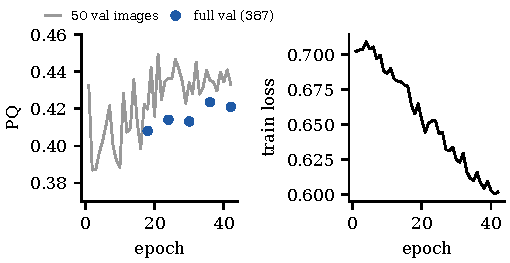
\includegraphics[width=\columnwidth]{fig_training.pdf}
\caption{Validation PQ (left) and training loss (right) of the final model per epoch.}
\label{fig:training}
\end{figure}

\begin{figure}[t]
\centering
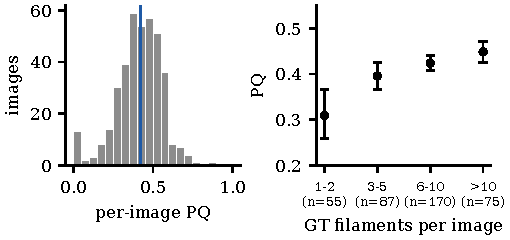
\includegraphics[width=\columnwidth]{fig_val.pdf}
\caption{Left: distribution of per-image PQ on the validation split (line: median). Right: PQ by number of ground-truth filaments per image with 95\% bootstrap intervals.}
\label{fig:val}
\end{figure}

\subsection{Test-time augmentation}\label{sec:tta}
    We evaluated TTA with the same weights and post-processing: the image is passed through the network in four views (identity, horizontal and vertical flips, rotation by 180$^\circ$) or eight views (all dihedral transforms), each soft mask is mapped back to the original orientation, and the candidates of all views are pooled before filtering and duplicate merging. All three settings were scored from the same forward passes on the full validation split and submitted to the leaderboard (Table~\ref{tab:tta}). TTA finds more filaments (95 more true positives with eight views) but adds 553 false positives and almost doubles the number of split filaments (82 to 150). A likely reason is that detections of the same filament from different views cover different parts of it and overlap by less than the merge threshold, so the overlap removal cuts the filament into pieces instead of merging them. Both the validation PQ and the leaderboard score decrease with the number of views, so the final submission uses a single view, which also needs one forward pass instead of eight.

\begin{table}[t]
\caption{Inference settings with the same weights. Validation: 387 images; LB: public leaderboard.}
\label{tab:tta}
\small
\begin{tabular}{@{}lrrrrrr@{}}
\toprule
Views & Home PQ & TP & FP & FN & Splits & LB PQ \\
\midrule
\textbf{1 (final)} & \textbf{0.4235} & 1912 & 1278 & 921 & 82 & \textbf{0.37} \\
4 & 0.4126 & 1982 & 1640 & 851 & 136 & 0.36 \\
8 & 0.4047 & 2007 & 1831 & 826 & 150 & 0.35 \\
\bottomrule
\end{tabular}
\end{table}


\subsection{Strengths, weaknesses and possible improvements}
    \textit{Strengths.} The model segments each filament as one instance in most cases (82 splits and 63 merges against 1912 matches), and the overlap removal guarantees a valid submission without manual cleaning. Training and inference run on a single 16~GB GPU.

    \textit{Weaknesses.} False positives outnumber false negatives (1278 vs.\ 921), so the model is tuned towards recall more than the metric rewards. Matched masks still differ from the annotations at the boundaries (mean IoU 0.667); the working resolution of 1344~px instead of 2048~px limits how well thin structures can be traced. The validation PQ is 0.05 higher than the public leaderboard score; a similar gap was observed for v2 (0.391 vs.\ 0.34), and we have no direct explanation for it. Gains between v3 and v5 (0.007 PQ) are smaller than the spread between neighbouring full-validation checkpoints (0.408--0.423), so we do not claim that the v5 changes are significant.

    \textit{Improvements.} (1) A higher detection-score threshold or a learned rescoring of the candidates should reduce false positives; TTA would need a merge rule that joins partial detections of the same filament instead of cutting them. (2) Inference on overlapping tiles at full 2048~px resolution would help thin structures. (3) Using the agreement between annotators of the same observation as soft targets could reduce the influence of annotation noise.

\section{Acknowledgment}\label{sec:acknowledgment}
    % Do not change
    The organization of the Filament Segmentation Challenge 2026 is partially supported by the U.S. National Science Foundation (NSF) under Grant No. 2209912 and 2433781, directorate for Computer and Information Science and Engineering (CSE), and Office of Advanced Cyberinfrastructure (OAC), and Grant No. 2511630, AST Division Of Astronomical Sciences and MPS Directorate for Mathematical and Physical Sciences.

    The Filament Segmentation Challenge 2026 is sponsored by the U.S. National Science Foundation (NSF) National Solar Observatory (NSO).

    This work utilizes GONG data obtained by the NSO Integrated Synoptic Program, managed by the National Solar Observatory, which is operated by the Association of Universities for Research in Astronomy (AURA), Inc. under a cooperative agreement with the National Science Foundation and with contribution from the National Oceanic and Atmospheric Administration. The GONG network of instruments is hosted by the Big Bear Solar Observatory, High Altitude Observatory, Learmonth Solar Observatory, Udaipur Solar Observatory, Instituto de Astrofísica de Canarias, and Cerro Tololo Interamerican Observatory.

\bibliographystyle{ACM-Reference-Format}
\bibliography{main}

\end{document}
